\documentclass[a4paper]{article}
\usepackage{graphicx}
\usepackage{multicol}
\usepackage{amsmath}
\usepackage{titlesec}

\graphicspath{ {./} }

\author{Braydan Newman: n11272031}
\title{MXB261 Problem-Solving Task}

\begin{document}
\maketitle
\tableofcontents

\newpage

\section{Part 1 - A Biased Random Walk}

\subsection{Single vs Random Starting Point}
 As show in Figure 1 and 2, having a single starting point vs a random starting point changes the distribution of column heights drastically.

\begin{figure}[h!]
  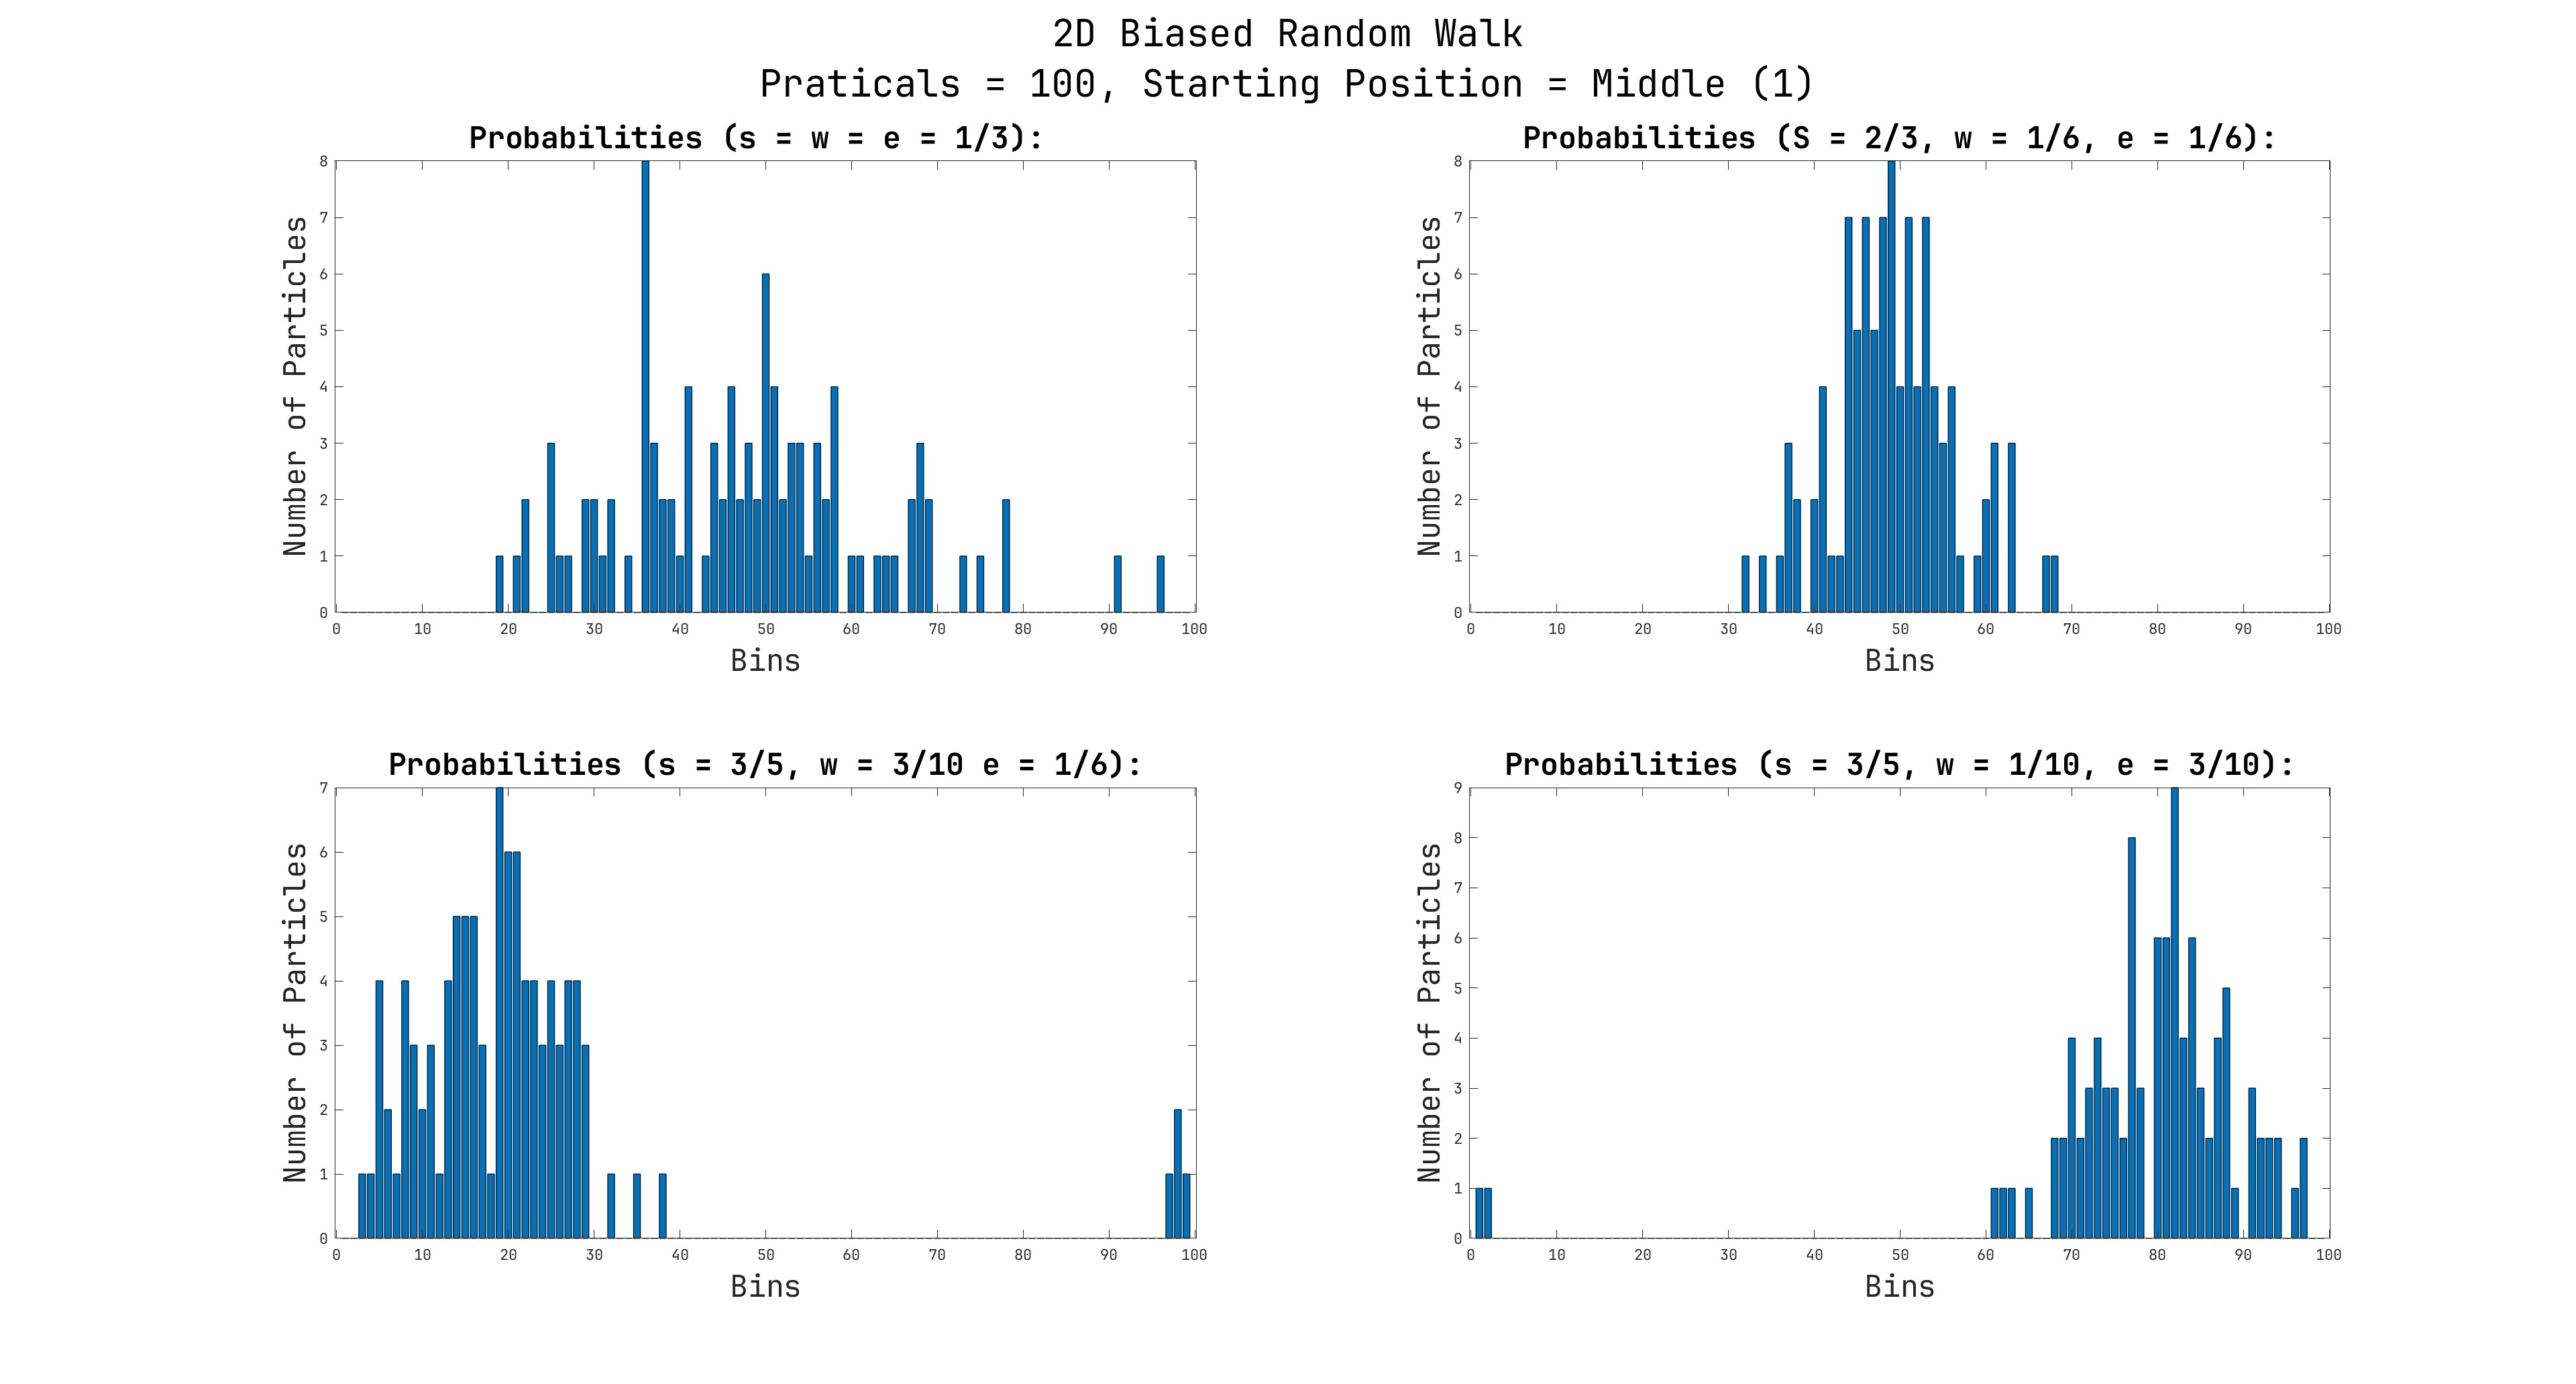
\includegraphics[width=\textwidth]{part1/p1_figure1}
  \caption{Middle Starting Position - 100 particles}
  \label{fig:msp}
\end{figure}

\begin{figure}[h!]
  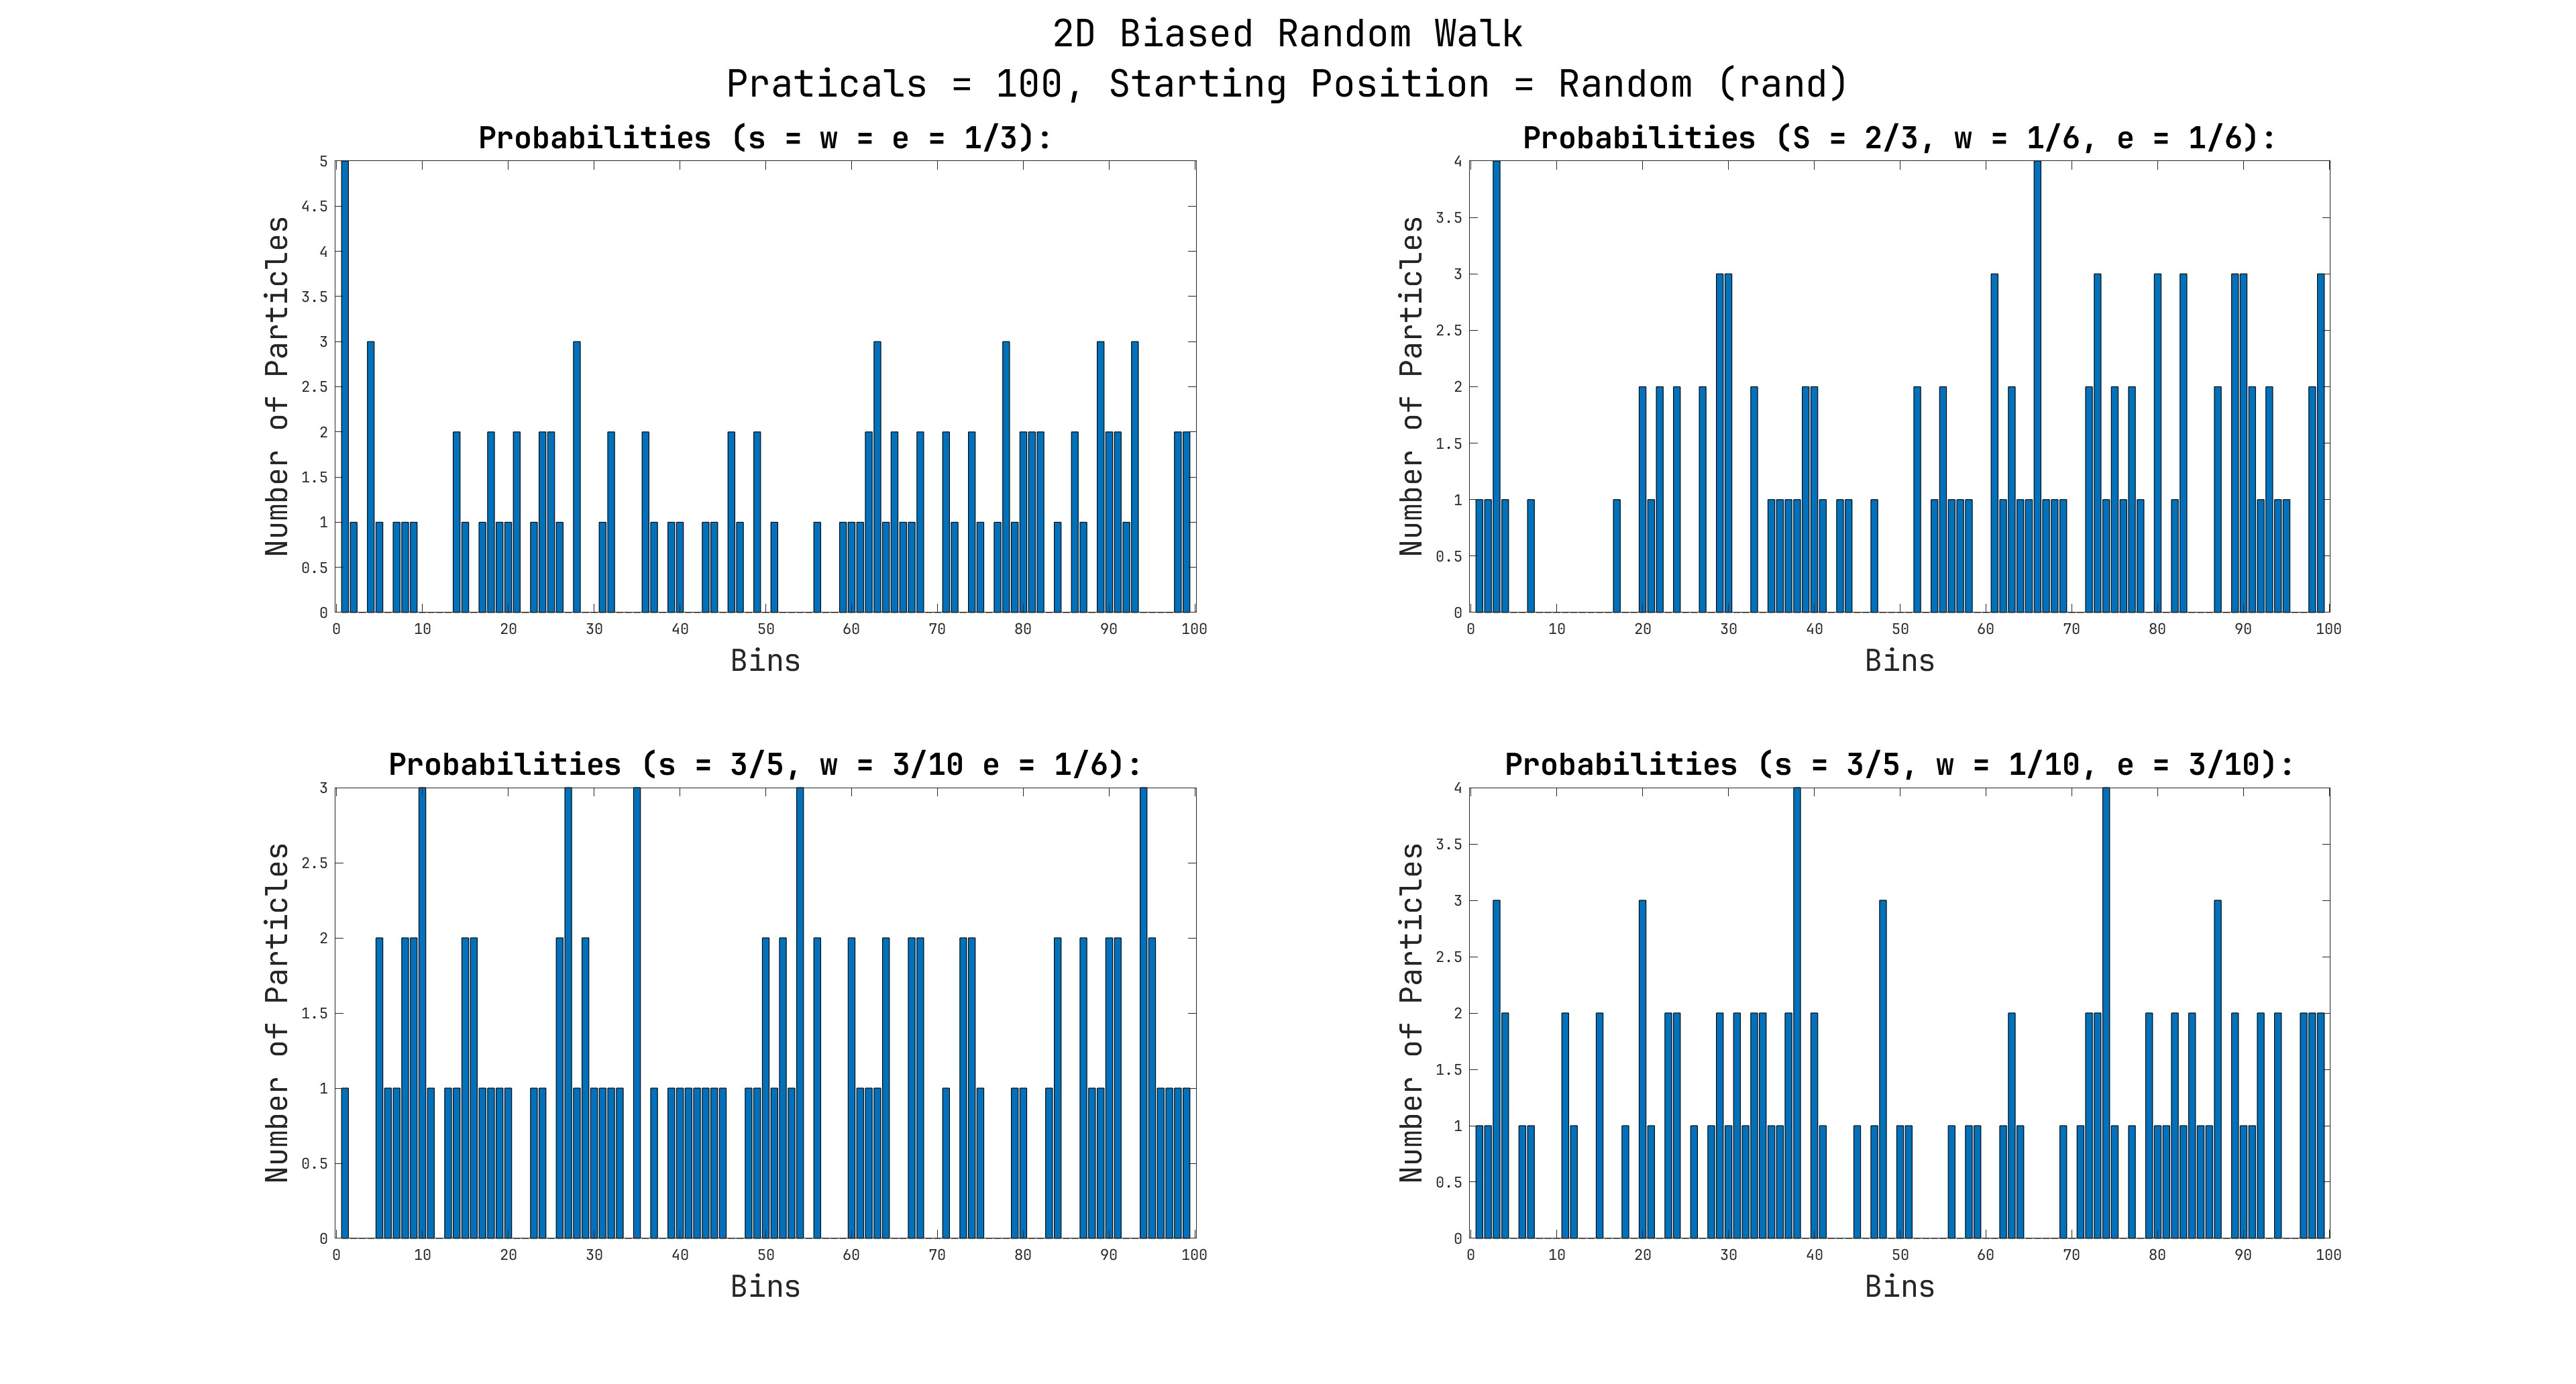
\includegraphics[width=\textwidth]{part1/p1_figure3}
  \caption{Random Starting Position - 100 particles}
  \label{fig:rsp}
\end{figure}

\newpage
Figure 1 shows distinct groupings of particle locations while Figure 2 shows no real discernible groupings of particles, and is spread out evenly with all column heights within 4 particles of each other. This shows that because of the randomness of the start position, the end location will be just as random even with the different biases in the directions. This could change if the simulation area didn't wrap around. The middle start position showed a strong tendency for all the particles to fall together, as the biases in the direction add together over many particles to increase the likelihood of a particle falling in a particular area.

\subsection{Increasing the Particles Count}
Increasing the particle count in the simulations does not change much in terms of the overall shape and distribution. Both the random and middle starting position have the same falling patterns as there respective 100 particle simulations and adding more particles doesn't change this. If the particle count was much smaller for the middle simulation, this would cause the graph to look a lot more random as the small differences between groups, or trivial correlations, would be detected as being statistically significant. However adding more particles makes the groupings more defined as shown in Figure 3. This is because with more data samples this reduces the amount of noise caused by the randomness. This is also shown in the random start position simulation (Figure 4), where the graph becomes much more level and flat, and with more particles this will continue to flatten out and become a uniform height across the whole graph.

\begin{figure}[h!]
  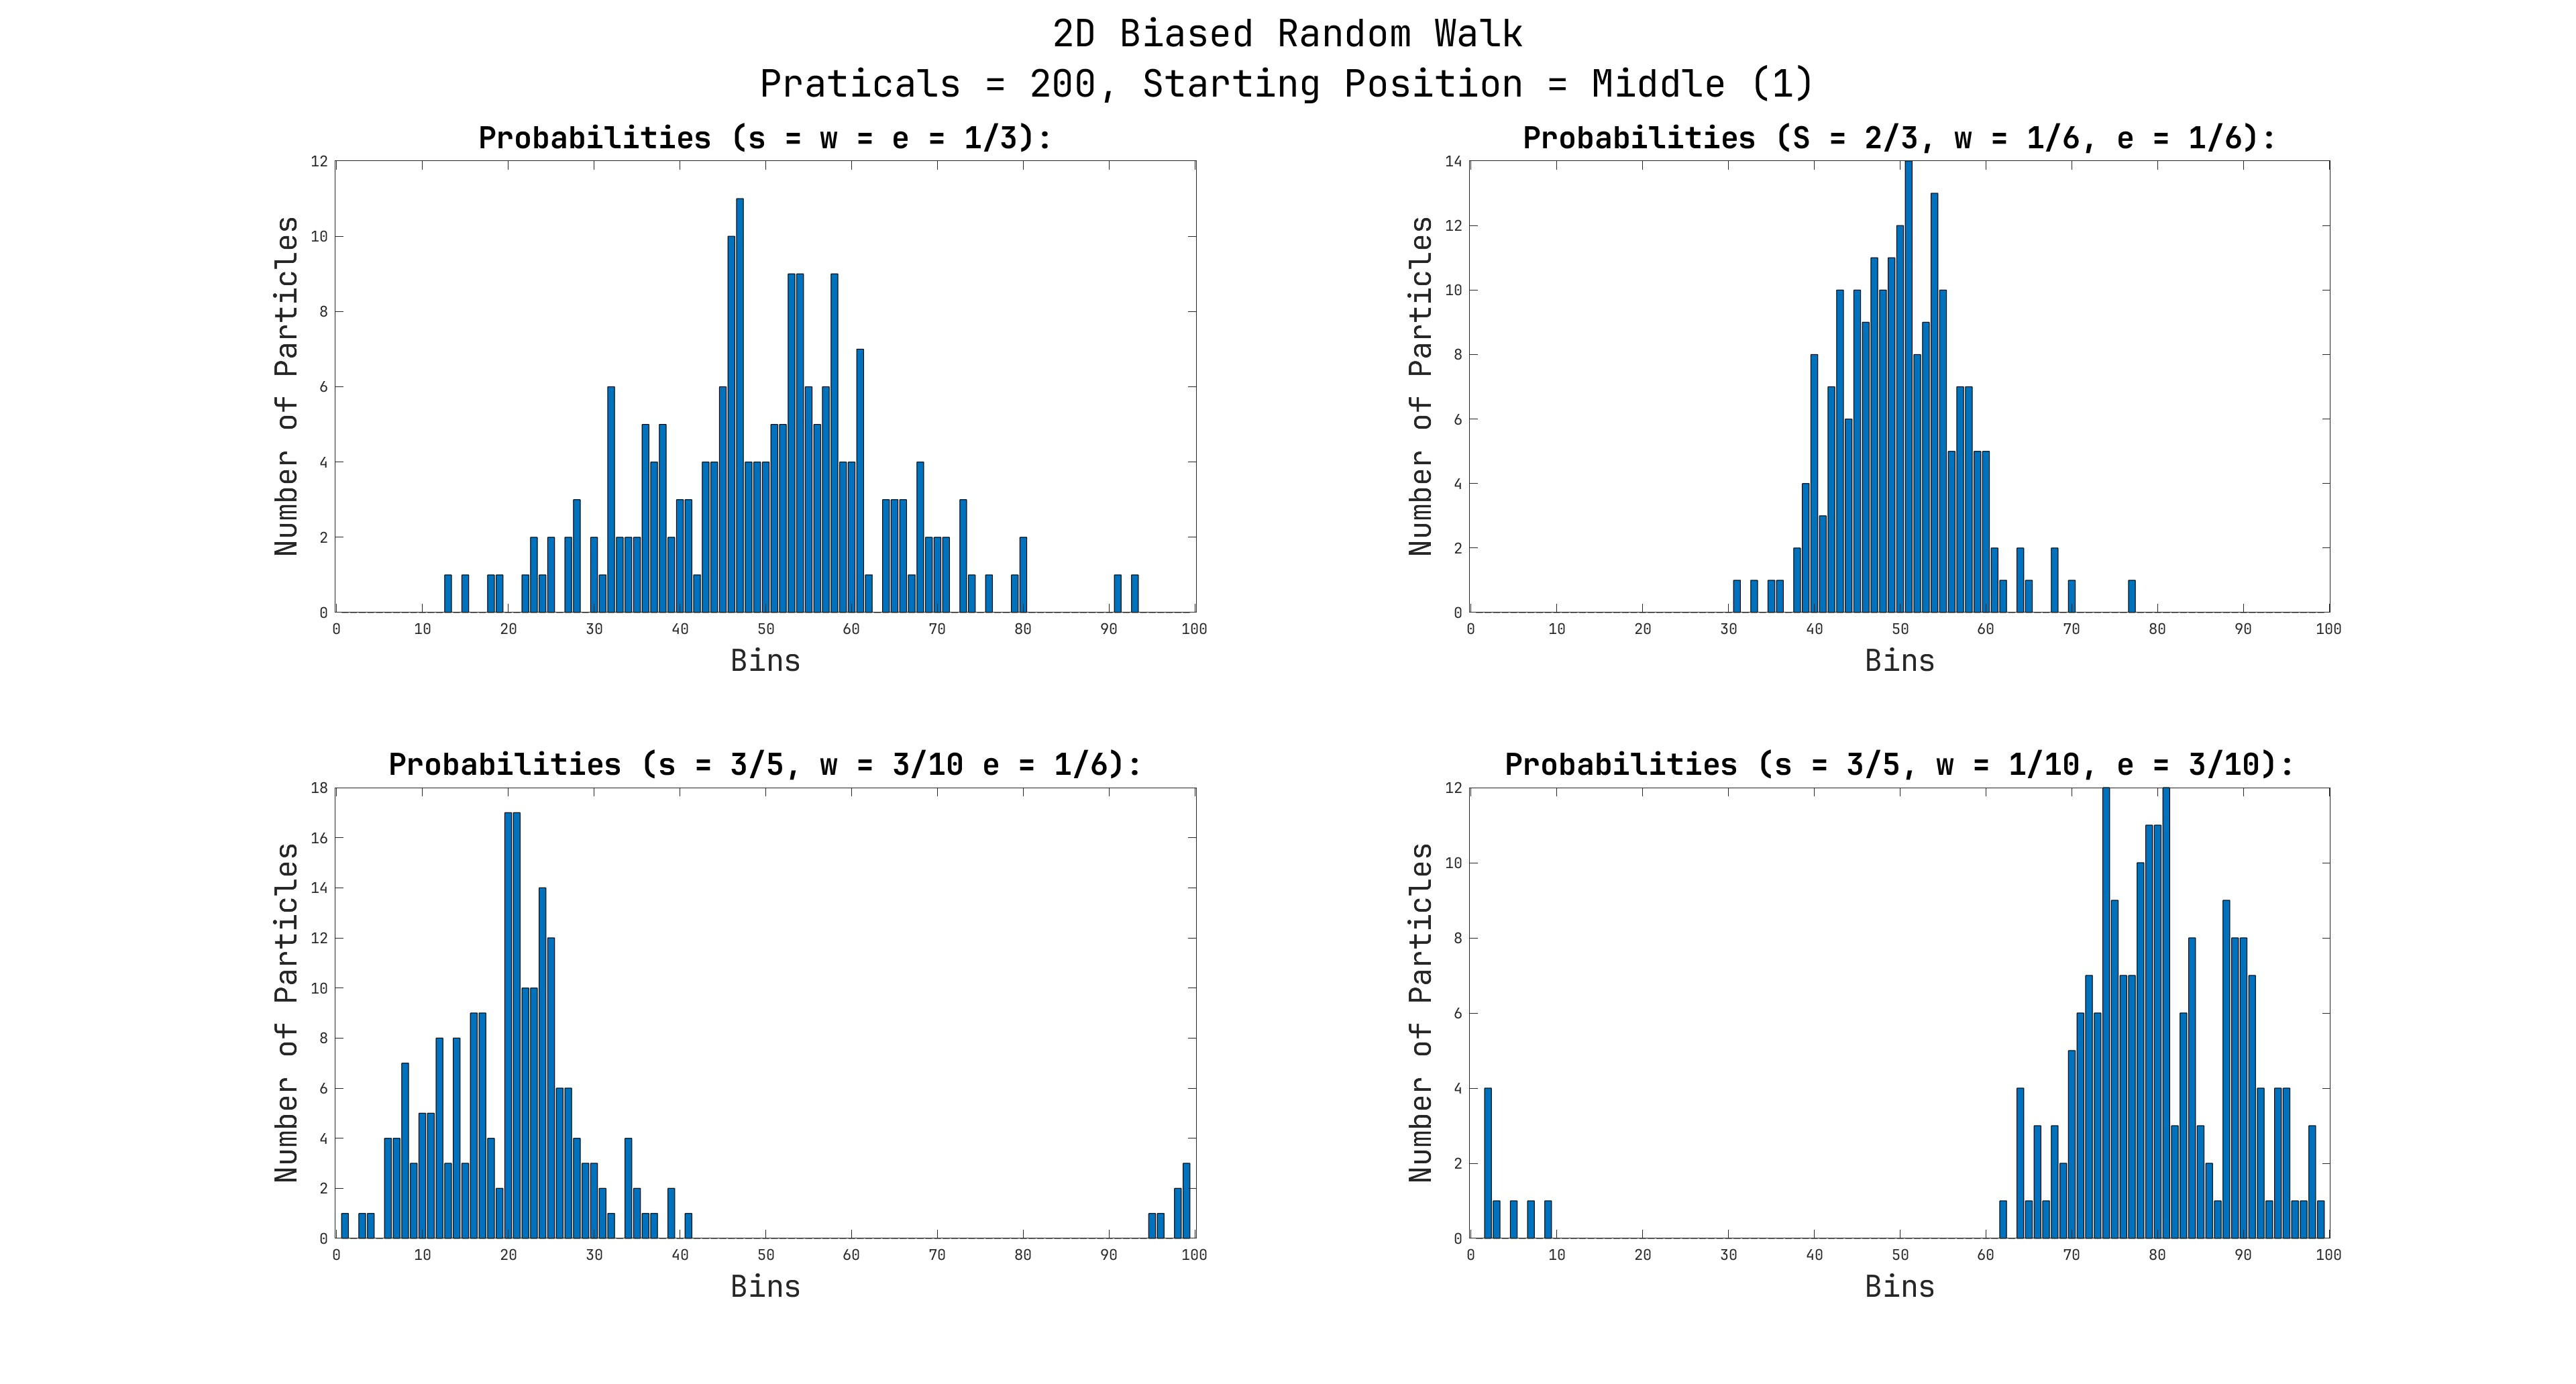
\includegraphics[width=\textwidth]{part1/p1_figure2}
  \caption{Middle Starting Position - 200 particles}
  \label{fig:msp200}
\end{figure}

\begin{figure}[h!]
  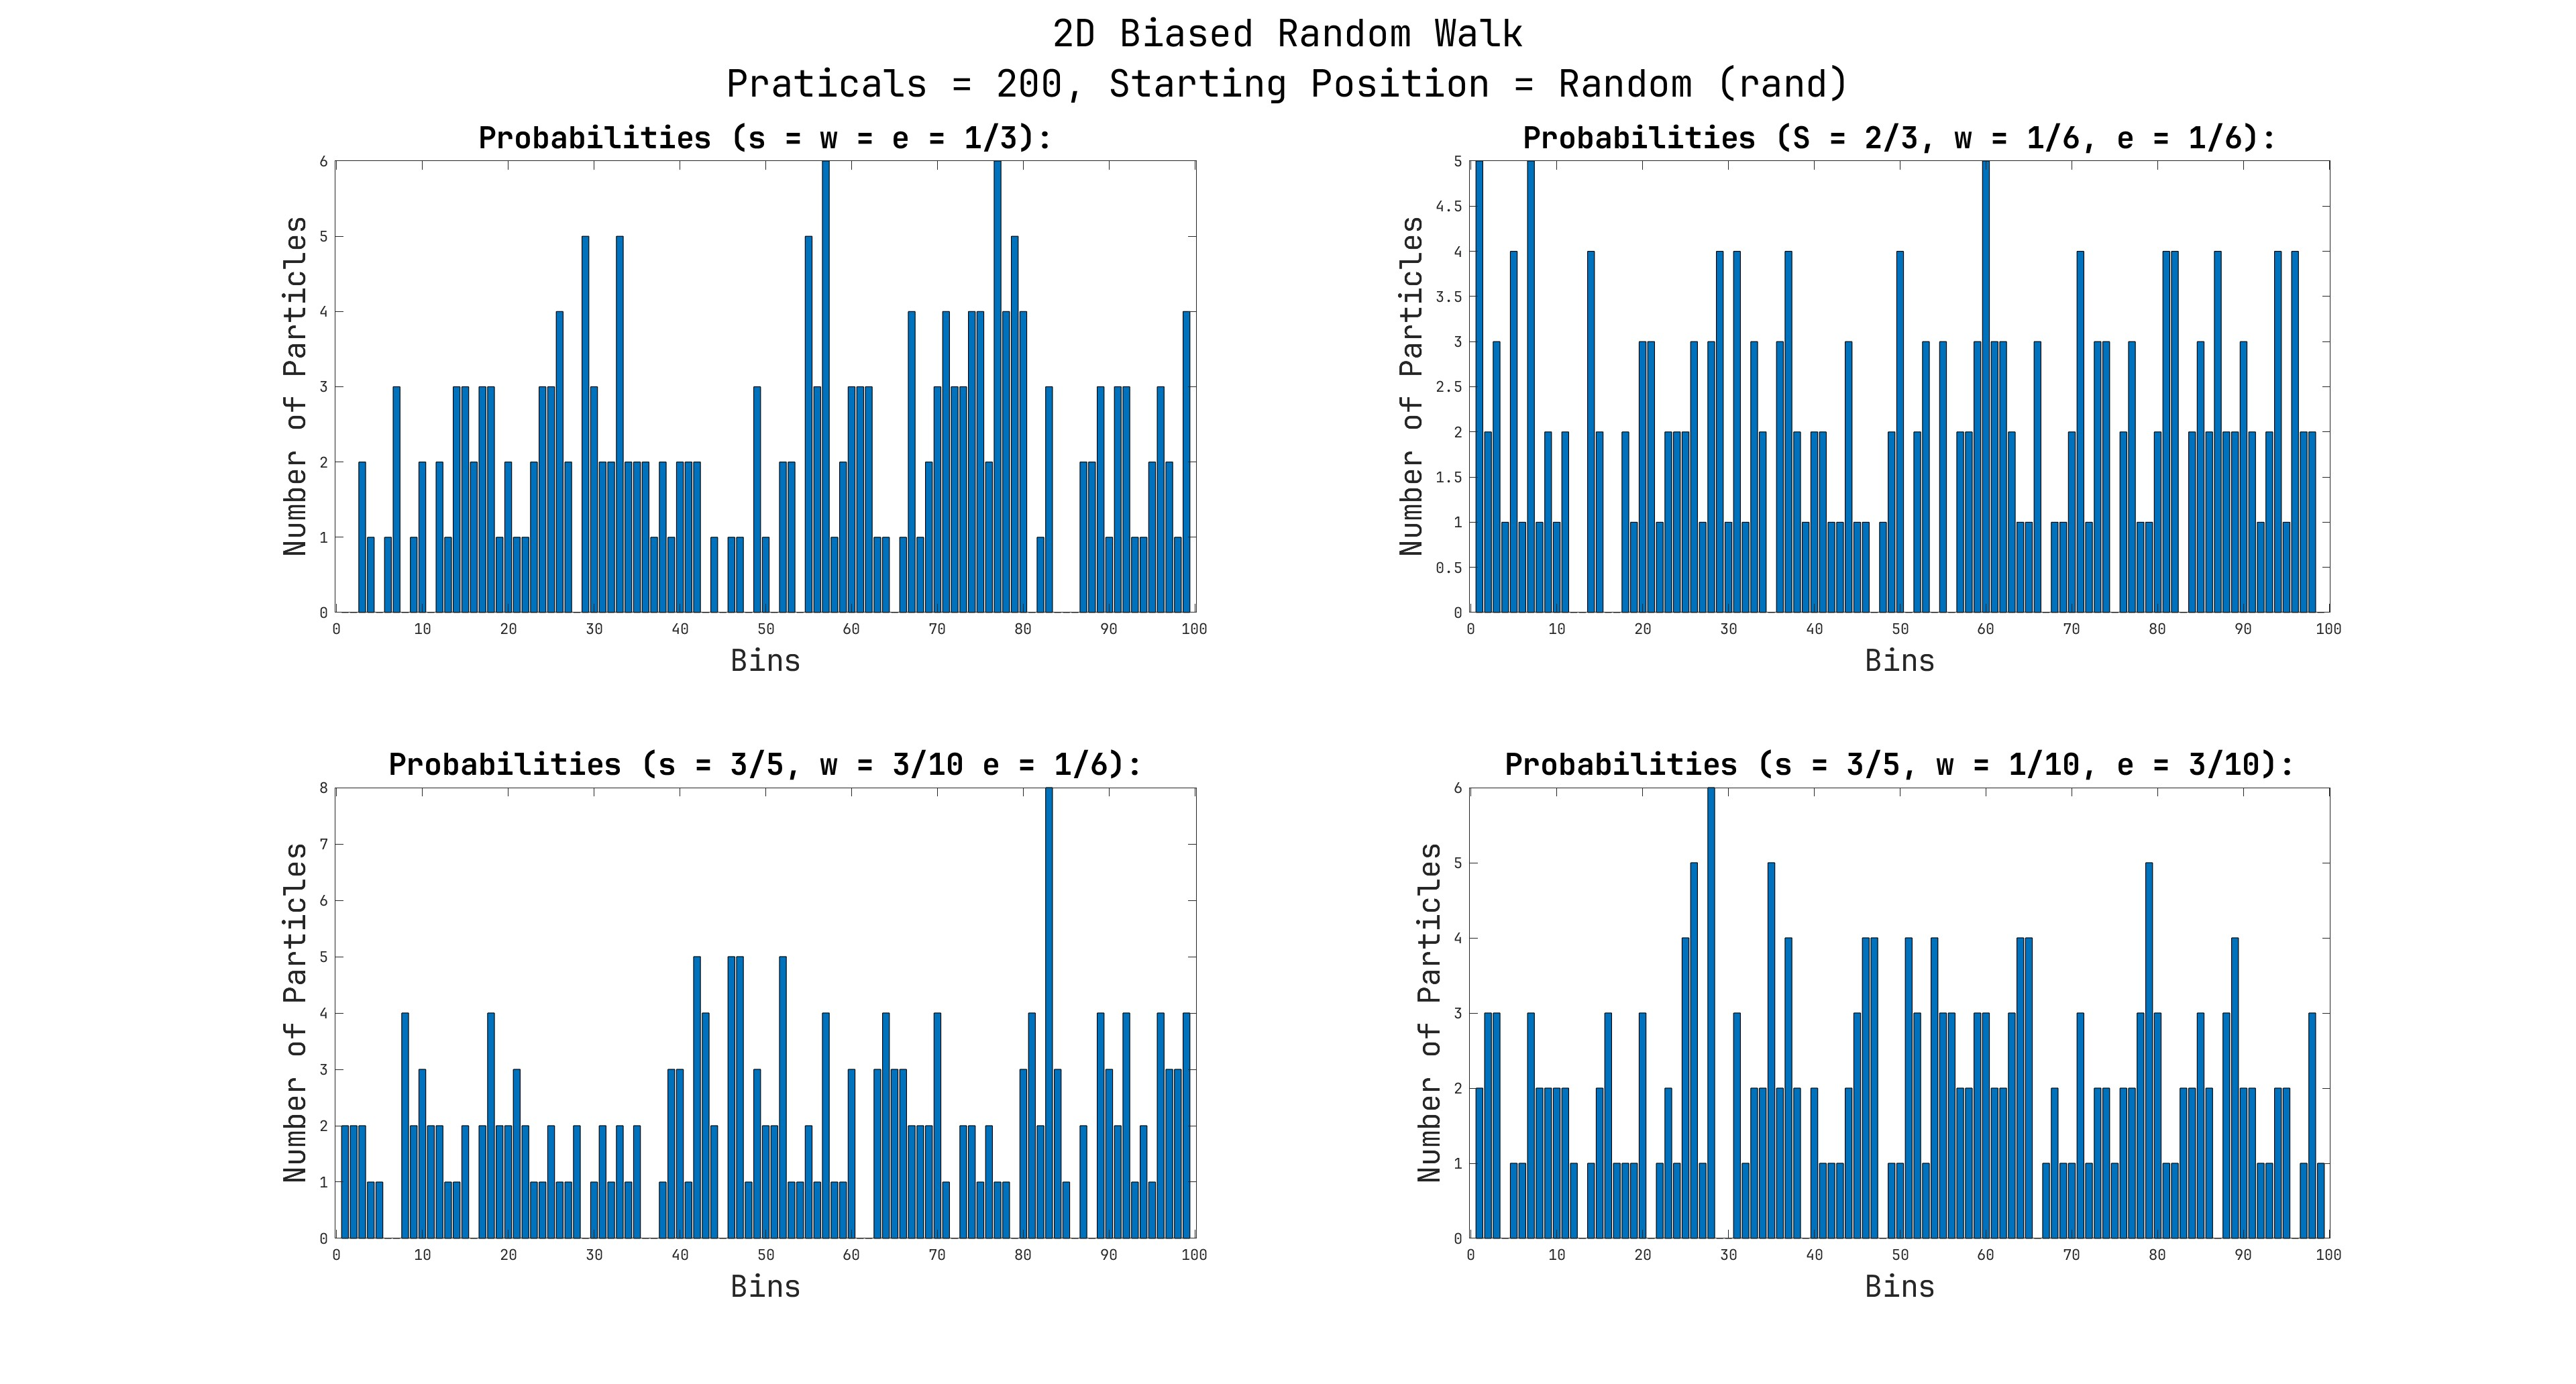
\includegraphics[width=\textwidth]{part1/p1_figure4}
  \caption{Random Starting Position - 200 particles}
  \label{fig:rsp200}
\end{figure}

\newpage

\subsection{Observations on the Distribution of Particles}
The middle starting position simulations all approximates a normal distribution, this is shown best by looking at the top left subplot in Figure 3 where all directions have equal probability. While the top left is shows a unit normal distribution all the other subplots for all simulations with the middle starting position are normal distribution too. These subplots just have different Skewness and kurtosis values.
\\
\\
This can been see more clearly when looking at the probability of the simulation area. This is a variation of this simulation with 2 possible directions instead of three, with equal probability for simplicity. Notice that the closer to the edges the less likely it is for the particle to make it there while vise verse in the center. The further down it goes the more prevalent it becomes.

\begin{figure}[h!]
  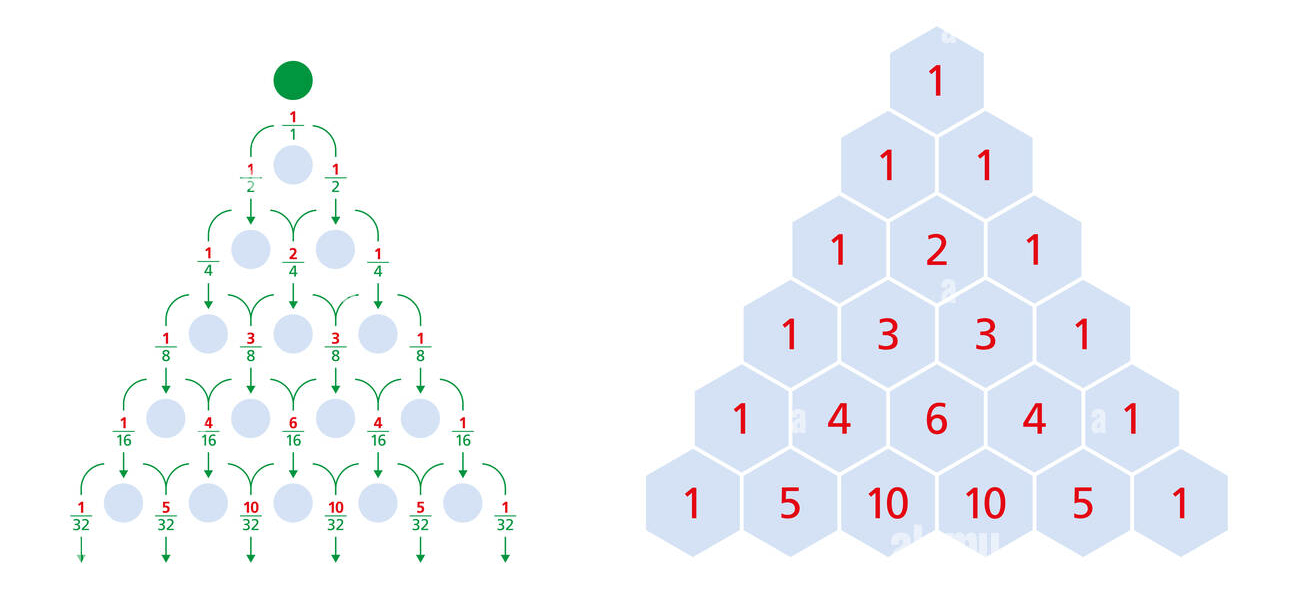
\includegraphics[width=\textwidth]{part1/galton-board-normal-distribution-and-pascals-triangle-a-triangular}
  \caption{Galton Board Normal Distribution and Pascals Triangle}
  \label{fig:rsp200}
\end{figure}

\newpage

\section{Part 2 - Sampling from Experimental Data}
\subsection{Similarities in the 2 Data Sets}
The data sets are very similar as seen in the probability distribution of the two dataset seen in Figure 6. They both follow basically the same pattern and this is to be expected. As the CDF used to sample data from to create the 2nd dataset was made with the 1st Dataset. The variation comes from the randomness of the samples collected. If more samples where collected it would converge on the first dataset.

\begin{figure}[h!]
  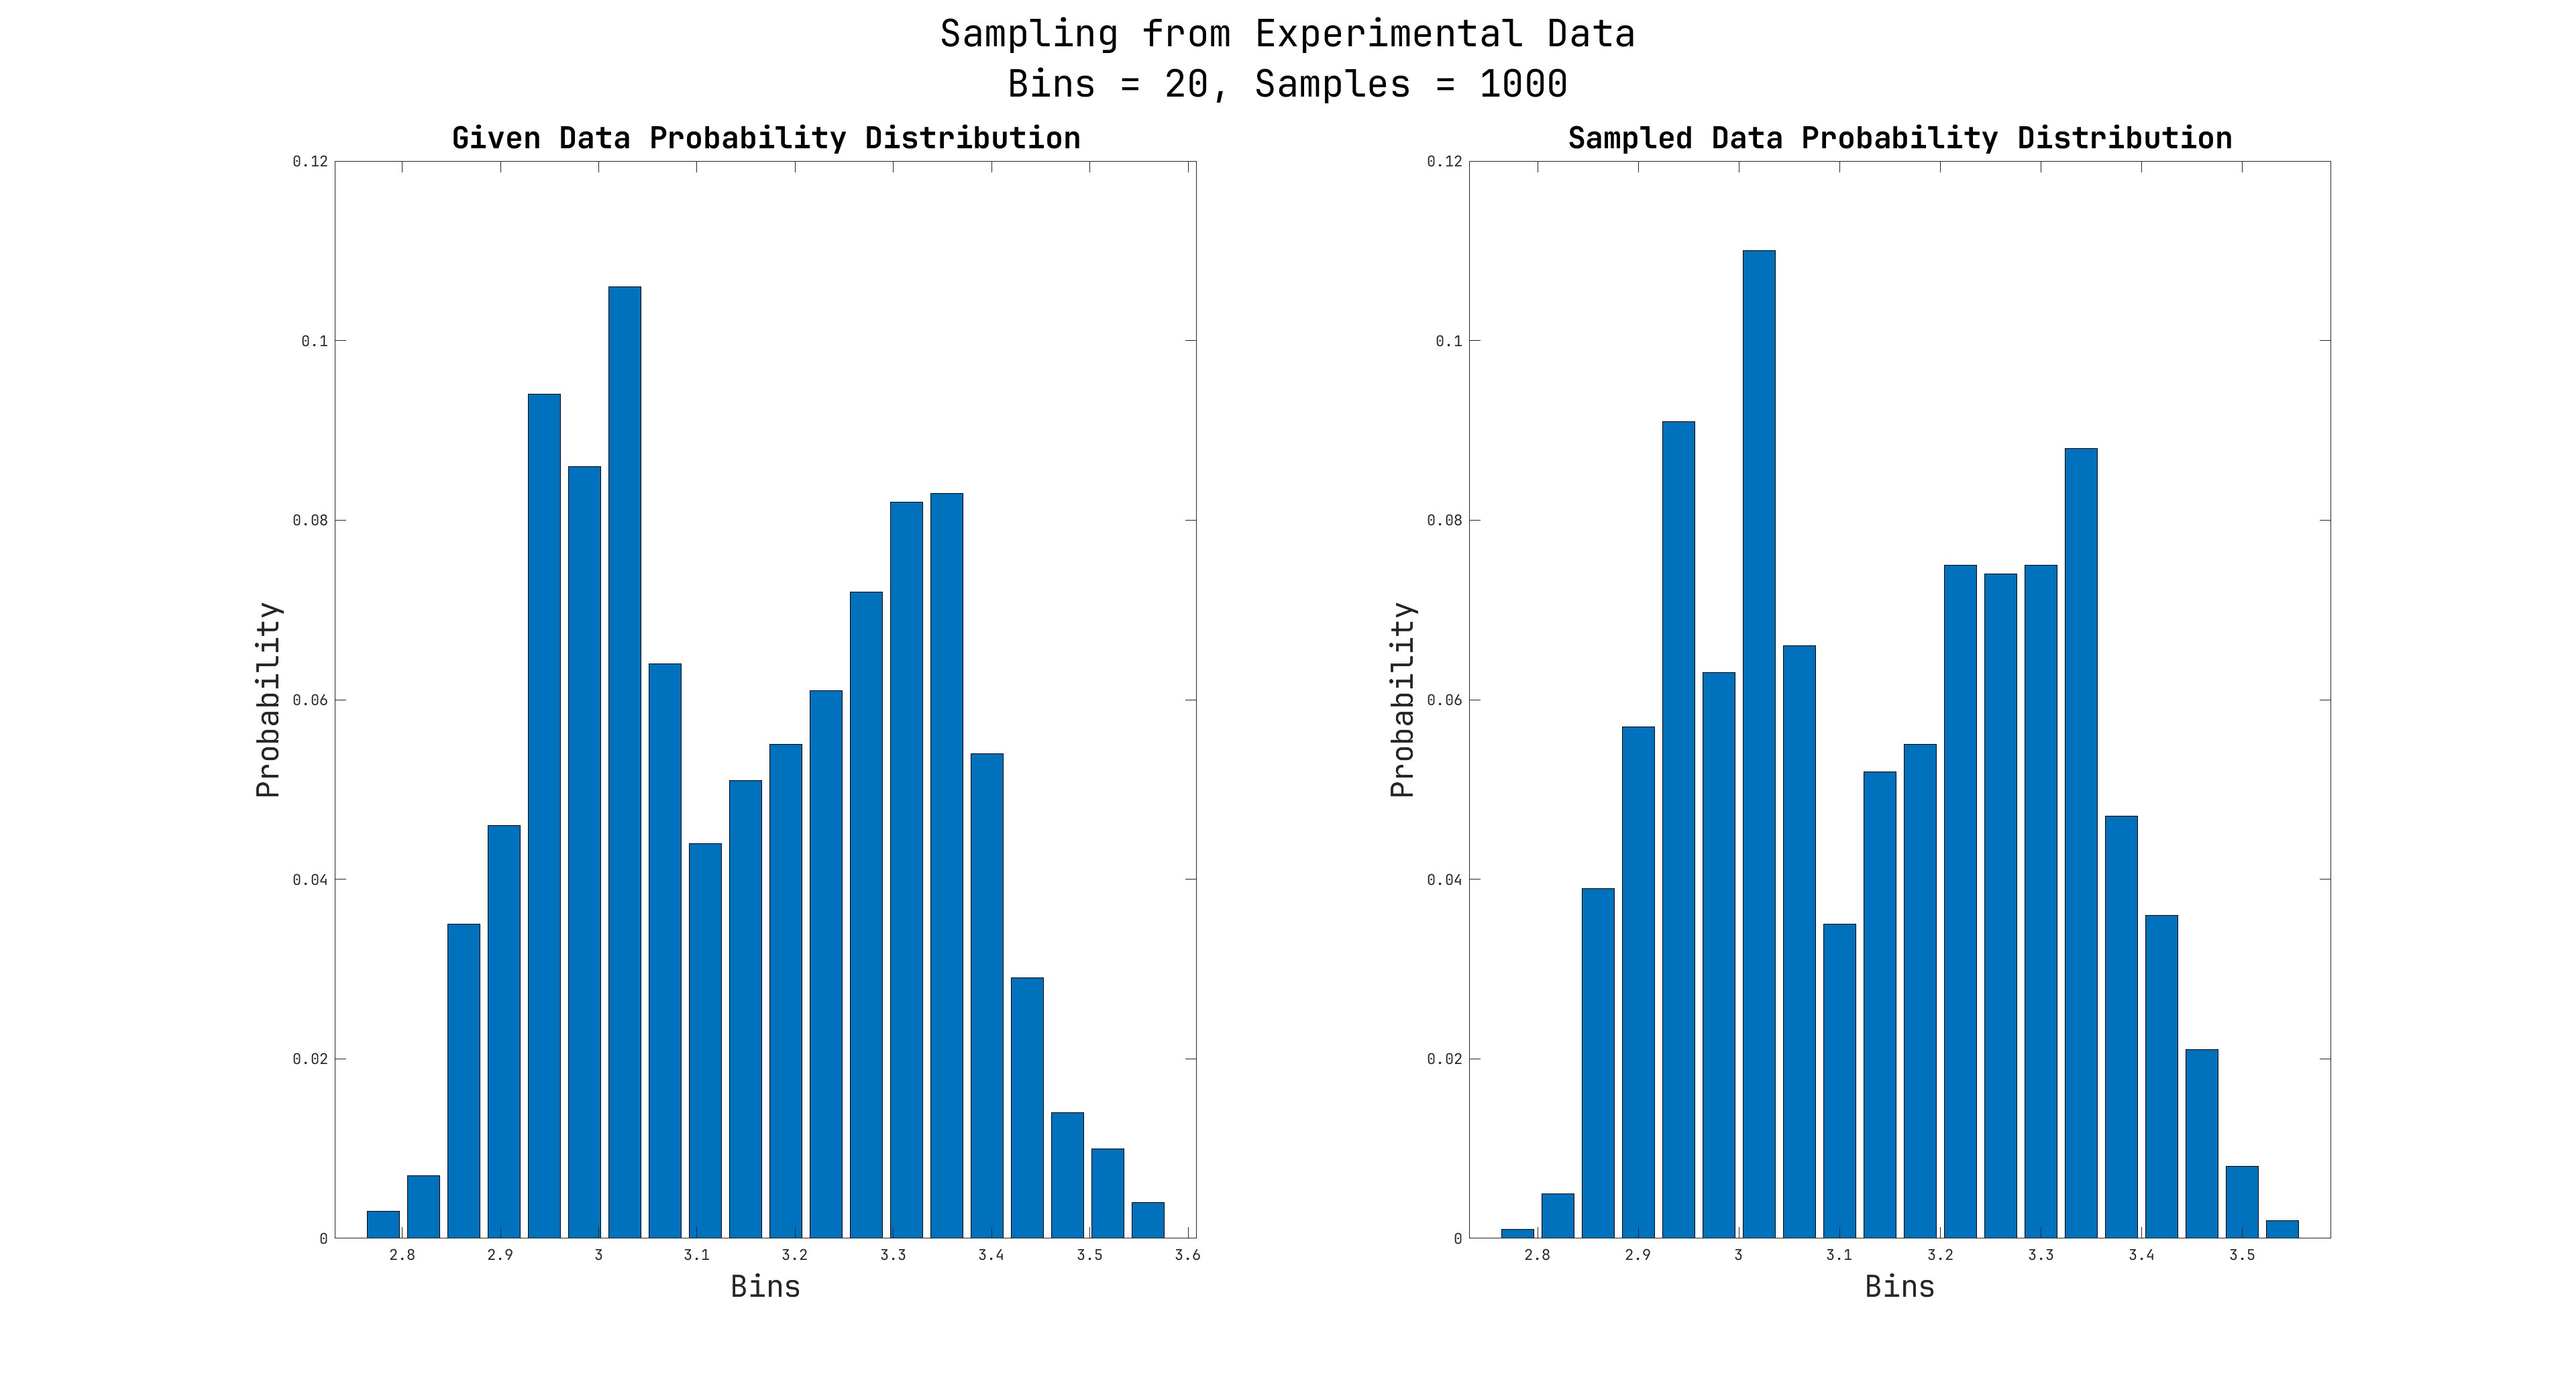
\includegraphics[width=\textwidth]{part2/figure1}
  \caption{Sampling from Experimental Data - 20 Bins}
  \label{fig:rsp200}
\end{figure}


\subsection{Kullback-Leibler Measurements on the Data Sets}
The Kullback–Leibler divergence, also known as relative entropy, is a a measure of how one probability distribution differs form another. 
\\\\
For the Datasets calculated with 20 Bins (Original and generated) the divergence can be different depending on which one you are measuring against, as seen in equation 1.

\begin{equation}
\begin{aligned}
  D_{KL}(P || Q) = 0.0134\\
  D_{KL}(Q || P) = 0.0128
\end{aligned}
\end{equation}\break
  
The K-L divergence of two random variables is an expected value, and so it matters which distribution you're taking the expectation with respect to.

\subsection{The Effect of Changing the Number of Bins}
The effect of changing the number of bins has a drastic effect of the Kullback-Leibler Measurement with a lower amount of bins the chance of having divergent bins is lower decreasing the Kullback-Leibler Measurement and vise verse for increasing the bin count.
\\
\\
This is shown in Figure 7 and Figure 8 where Figure 7 is the decreased bin count of 10 and Figure 8 has an increased bin count of 40. The amount of variations between the two subplot graphs is far higher in the 40 bin PDF then the far smaller amount of variations in the 10 bin PDF. This is proven in the Kullback-Leibler Measurements for both PDF's comparisons. 
\\
\\
(2) = 10 Bins - figure 7\\
(3) = 40 Bins - figure 8

\begin{multicols}{2}
  \begin{equation}
  \begin{aligned}
    D_{KL}(P || Q) = 0.0047\\
	D_{KL}(Q || P) = 0.0045
	\end{aligned}
  \end{equation}\break
  \begin{equation}
      \begin{aligned}
    D_{KL}(P || Q) = 0.0184\\
	D_{KL}(Q || P) = 0.0178
	\end{aligned}
  \end{equation}
\end{multicols}
\begin{figure}[h!]
  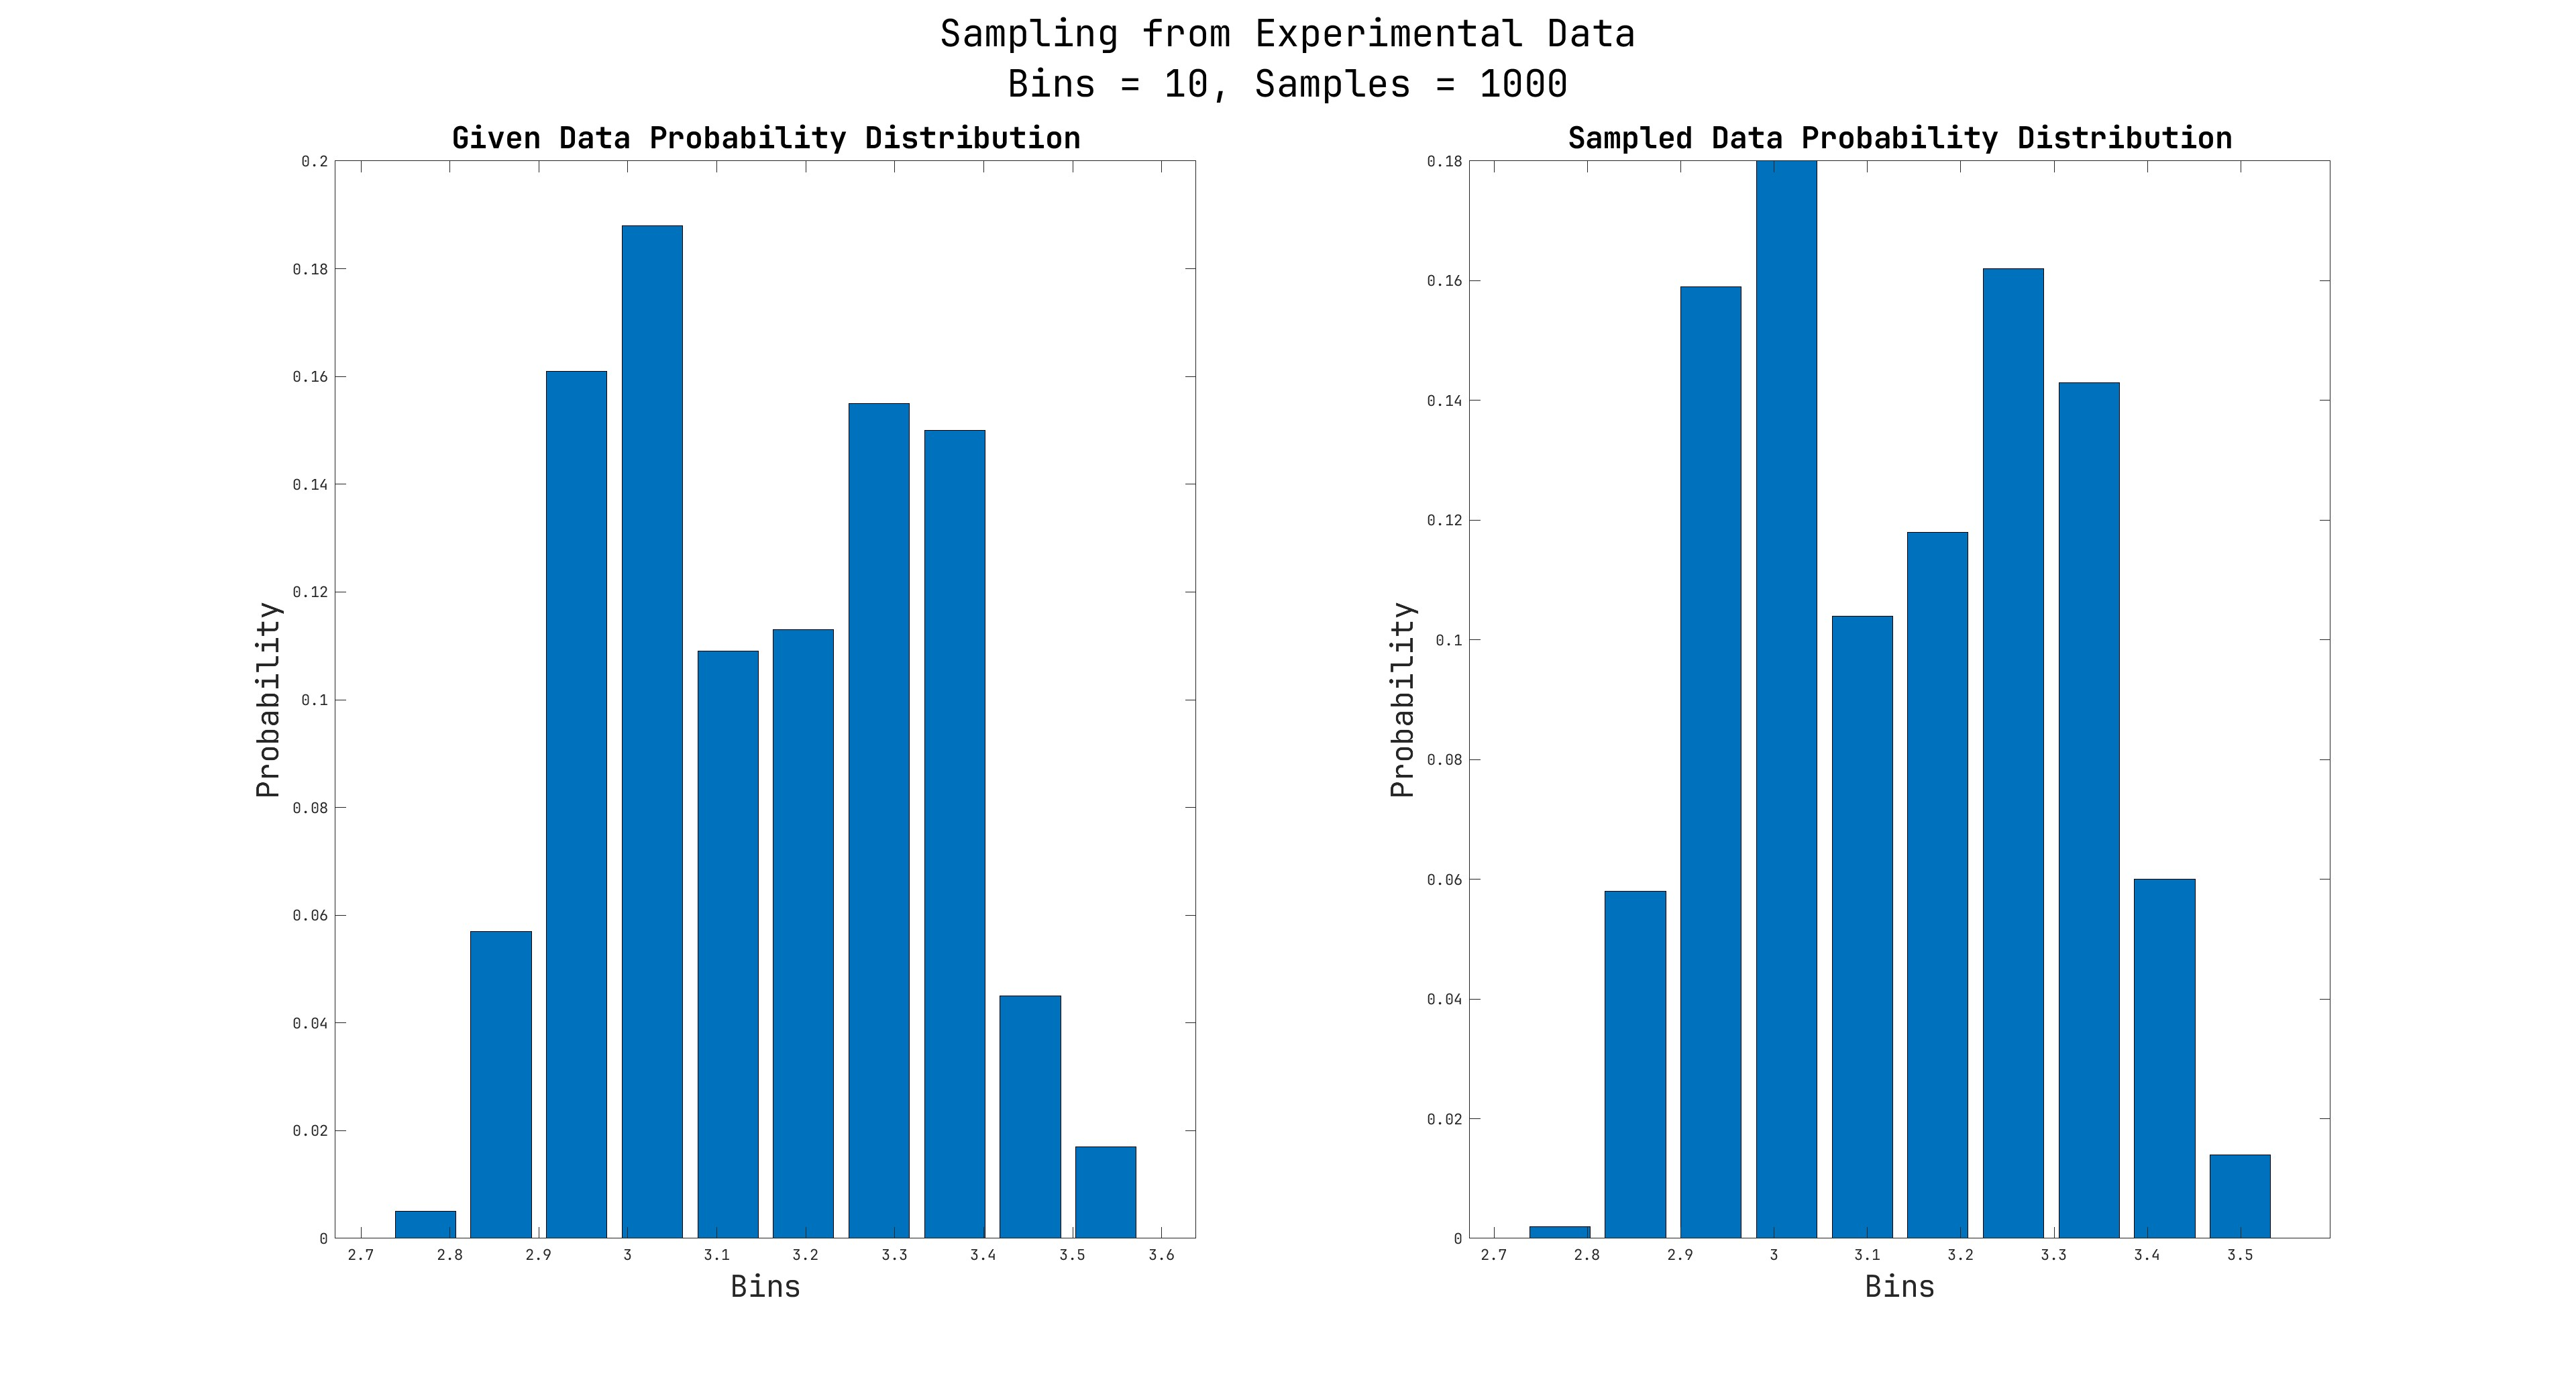
\includegraphics[width=\textwidth]{part2/figure2}
  \caption{Sampling from Experimental Data - 10 Bins}
  \label{fig:rsp200}
\end{figure}
\begin{figure}[h!]
  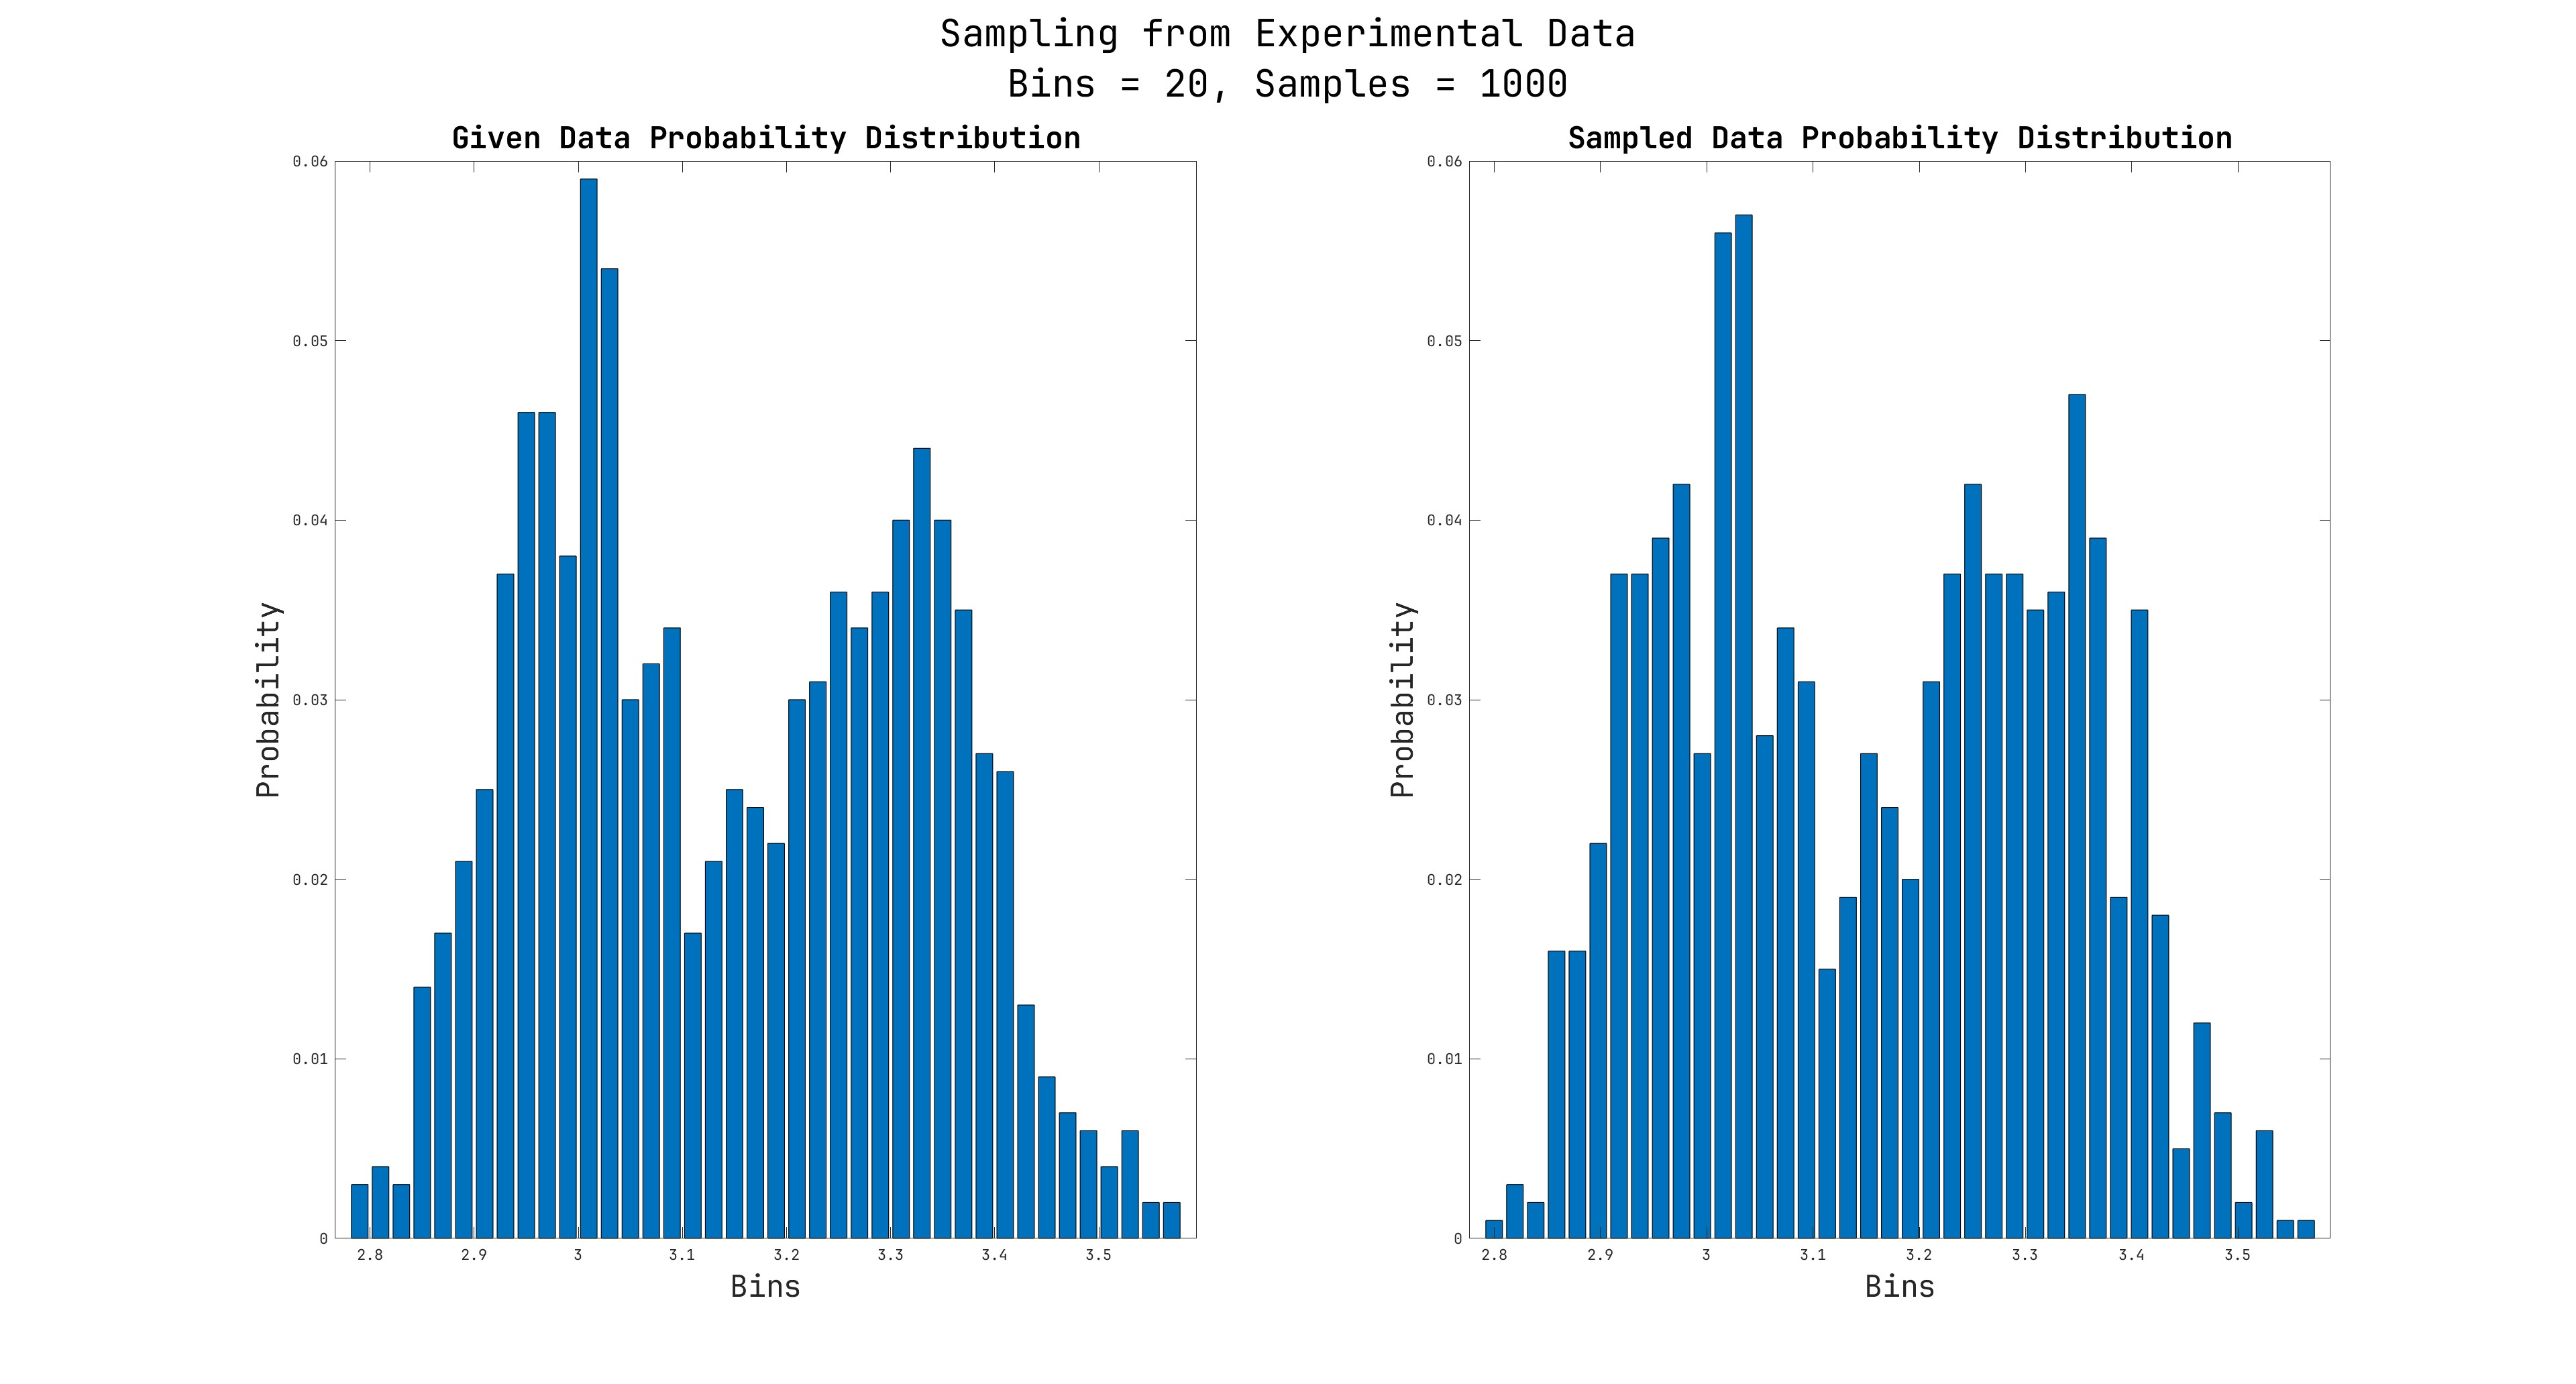
\includegraphics[width=\textwidth]{part2/figure3}
  \caption{Sampling from Experimental Data - 40 Bins}
  \label{fig:rsp200}
\end{figure}
\end{document}